% 公立はこだて未来大学 卒業論文 テンプレート ver1.50
% (c) Junichi Akita (akita@fun.ac.jp), 2003.10.31
% update by N.T.,  2004.11.10
%
\documentclass{funthesis}
%\documentclass[english]{funthesis} % use [english] option for English style

%\usepackage{graphicx} % 図(EPS形式)を本文中で読み込む場合はこれを宣言
\usepackage[dvipdfmx]{graphicx}
\graphicspath{{./img/}}
\usepackage{here}

% この部分に,タイトル・氏名などを書く.
% タイトルなどの定義の始まり
\jtitle{Leap Motionによる教育をインタラクティブにするシステムの提案\\
%--- 一二三四五六七八九十 ---
}  % 論文の和文タイトル
%
\etitle{Title in English\\
--- one two three four five six seven eight nine ten ---
}% 論文の英文タイトル
%q
\htitle{Short Title in English}   % ヘッダー用の論文の短縮英文タイトル
%     必ず1行に収まるように英文タイトルを短縮する.
%
\jauthor{一ノ瀬 智太}     % 氏名(日本語)
\eauthor{Tomohiro Ichinose }   % 氏名(英語)
\jaffiliciation{情報アーキテクチャ学科} % 所属学科名(日本語)
\eaffiliciation{Department of Complex Media Architecture} % 所属学科名(英語)
\studentnumber{1012211}   % 学籍番号
\jadvisor{美馬 義亮}    % 正指導教員名(日本語)
%\jcoadvisor{副指導 教員} % 副指導教員(日本語)がいる場合は
                        % コメントアウトし名前を書く
                        % 副指導教員がいない場合は,ここは削除しても可
\eadvisor{Prof. Advisor}  % 正指導教員名(英語)
\ecoadvisor{Prof. Coadvisor}   % 副指導教員(英語)がいる場合は
                         % コメントアウトし名前を書く
                         % 副指導教員がいない場合は,ここは削除しても可
\jdate{2016年1月29日}    % 論文提出日   (日本語)
\edate{January 29, 2016}     % 論文提出年月 (英語)
% タイトルなどの定義の終わり

\begin{document}

%--------------------------------------------------------------------
\maketitle       % タイトルページを作成

%--------------------------------------------------------------------
% 英文概要(250語程度)
\begin{eabstract}
Teachers use a blackboard and chalk in the field of school education. On the other hand, students use pencil and notebook was mainstream. However, classes that use a personal computer and tablet devices have been introduced in recent years. It is that the exchanges of the information from a teacher to a student are unilateral to be common when I compared the recent school education with the conventional thing. In this study, the purpose is to implement an application for realizing interactive teaching operations between teachers and students in the field of education, and evaluate usefulness.
\end{eabstract}

% 英文キーワード(5個程度をコンマ(,)で区切って羅列する)
\begin{ekeyword}
Keyrods1, Keyword2, Keyword3, Keyword4, Keyword5
\end{ekeyword}

%--------------------------------------------------------------------
% 和文概要(400字程度)
\begin{jabstract}
学校教育の場において教師は黒板とチョークを使い, 学生は鉛筆やノートを使った授業が主流であった. しかし, 近年ではパーソナルコンピュータやタブレット端末を使った授業が取り入れられている. 近年の学校教育を従来のものと比較した際に共通することは,教師から学生への情報のやり取りが一方的なことである.本研究では, 教育の場において教師と学生間での対話的な授業運営を実現するためのアプリケーションを実装し,その有用性を評価することを目的とする.

\end{jabstract}

% 和文キーワード(5個程度をコンマ(,)で区切って羅列する)
\begin{jkeyword}
キーワード1, キーワード2, キーワード3, キーワード4, キーワード5
\end{jkeyword}

%--------------------------------------------------------------------
\tableofcontents % 目次を作成


% 本文のはじまり
%--------------------------------------------------------------------
\chapter{序論} % 章のタイトル
%\chapter{Introduction} % sample of English style

% \includegraphics[width=??cm]{hoge.eps} % 図(EPS形式)を読み込む場合

\section{背景} % sectionのタイトル

% 以下に背景,関連する環境,状況,技術に関する概要を記述.

%ここはneeds
学制百年史 [1] によると日本における大学の誕生は明治時代に遡る.一斉授業の場において,教師は知識を与え学生はそれを吸収するというモデルに基づく. こうした場において, 一部の学生には頬杖をついたり, 居眠りをしたりなどが散見される. その原因として, 日々の生活の疲れだけでなく, 教師の説明が理解できず, 授業についていけないなどのストレスが挙げられる. こうした学生には他の学生に比べて学習意欲が低下しているといえる.\\
%ゼミでもカバーできるということを記述
大学のゼミにおいても同じである. 話し手が一方的に先に話し, 聞き手が質問...-


%一斉授業の形態として, 教師という話し手に対し,, 学生が聞き手である. 
%ゼミでの教師か学生が話し手でその他の学生と

%ここはseeds、技術的な変化
%新しいデバイス, ネットワークインフラの登場 → 学校内でLANが普及しネットが...
% 									  → LeapMotionを使う、PC、タブレット端末等を使うようになった
近年では, Leap Motionなどの新しいデバイスの登場や学校内でのLANが普及により, PCが身近なものになってきている. 


\section{目的}
本研究では, こうした学習意欲の低下を着目し, これを解決するために教師と学生の間に双方向性をもたせ,  学習意欲の向上を図ることを目的とする. その方法として, Leap Motionというセンサが手や指の位置, 方向, 曲げ, ジェスチャー等を検知できるセンサを用いて, 双方向性を実現するアプリケーションを実装し, 学習意欲が向上することを目指す. 具体的には学生が授業中に抱いている「助けてほしい」や「もう一度説明してほしい」などのメッセージをLeap Motionで入力し,教師に伝えるということをめざす. 
%もっと何をしたいのかを明確に記述する
%追記 ” 授業に大きな影響を与えることなく ” 

%\section{研究目標}


%--------------------------------------------------------------------
\chapter{問題設定・研究アプローチ} % 章のタイトル
%\chapter{Introduction} % sample of English style

\section{問題設定}
% \includegraphics[width=??cm]{hoge.eps} % 図(EPS形式)を読み込む場合

%言い回しが長くならないようにする
本研究での問題は一斉授業の場において双方向性を実現し, 学習意欲の向上を目指す. Leap Motion というセンサが手や指の動きを検知し入力操作を行い, その時に音を立てないのでこれを使用する. 本研究での一斉授業の場の位置付けとして, 教師と学生の双方がパーソナルコンピュータを使用していることを想定する. 具体的な例として, 教師はパーソナルコンピュータで資料をプロジェクターに投影しながら授業を行い, 一方, 学生はメモをとったり課題に取り組むために使用しているものとする.

% 以下に現状の問題・研究アプローチを記述.

\section{研究アプローチ}
ここでは実際のアプリケーションを使うときのシナリオを記述する. まず, 実際の授業の中で学生は「大きな声で話してほしい」や「もう一度説明してほしい」といった感情を抱く. これらの感情を Leap Motion を使ったアプリケーションで発信し, プロジェクターに投影する. その発信を基に教師がアクションを起こし, 対話的な授業運営を実現する. 一方で, 学生側の発信が多くなり過ぎた場合, 教師へのストレスが懸念される. 
%具体性が欲しい

%--------------------------------------------------------------------
\chapter{関連研究}
ここでは対話的授業運営の関連研究としてクリッカーを, 意思決定ツールとしてサイボウズLiveを取り上げる.
%グループウェアで検索してまだないか調べる

%コンセプトを絵にする
\section{クリッカー}
双方向性授業の実現としてクリッカー [4] を用いた事例がある. クリッカー(授業応答システム)とは赤外線リモコンによる学生解答システムである. 授業中に教師が問題を出し, 学生がクリッカーを用いて解答するというものである. クリッカーを用いた結果として,「役に立つ」という問いに対して「役に立つ」と答えた学生が 6 割を上回り,「勉強する気になったか」という問いに対しては「やる気が出た」という学生が 7 割を上回っている.
%どのように使うのかを記述
%本システムとの違いを描く
%画像の挿入
\subsection{提案するシステムとの違い}

\section{サイボウズLive[] }

%サイボウズ
%http://products.cybozu.co.jp/office/
%サイボウズlive
%https://live.cybozu.co.jp/overview.html

%サイボウズ社が開発した意思決定ツール
%主な機能
%導入事例とか...

サイボウズLive(\ref{cybozu})はサイボウズ社が開発した意思決定ツールである. 
主な機能として、以下の5つが紹介されている.
\begin{itemize}
 \item タイムライン:メンバーに聞きたいこと、伝えたいことを書く
 \item 掲示板:掲示板のコメント欄でメンバーとディスカッションする
 \item イベント:プロフェクトのイベントやスケジュールを登録・共有できる
 \item ToDoリスト:メンバーとToDoを共有できる
 \item 共有フォルダ:1グループにつき1Gバイトまで無料でファイルを保存可能
\end{itemize}
また, 2014年2月26日よりチャット機能が追加された. チャット機能の利点は以下の3つが紹介されている.\\
 1つ目は, PCでもスマートフォンでもメッセージがすぐ届く点である. サイボウズLiveのチャット機能はPCだけでなく, スマートフォンでも使うことできる. 投稿したコメントは相手の画面にただちに用事されるので, オンラインのミーティングがスムーズに行える. \\
 2つ目は,  複数人でも1対1でもチャットが出来る点である. 複数人のメンバーを指定して, チャットスペースを作成できる. また, サイボウズLive上で知人と繋がると, 自動的に1対1のチャットスペースが作成されるので, 簡単にチャットのやりとりをスタートできる. \\
 3つ目は,  グループ機能と併用すれば, 情報の整理が楽になるという点である. チャットのやりとりで決定したことは, 先に記述したToDoリストに登録しておくことができる. \\
%本システムとの違いを描く
\subsection{提案するシステムとの違い}


%画像の挿入
\begin{figure}[H]
 \begin{center}
  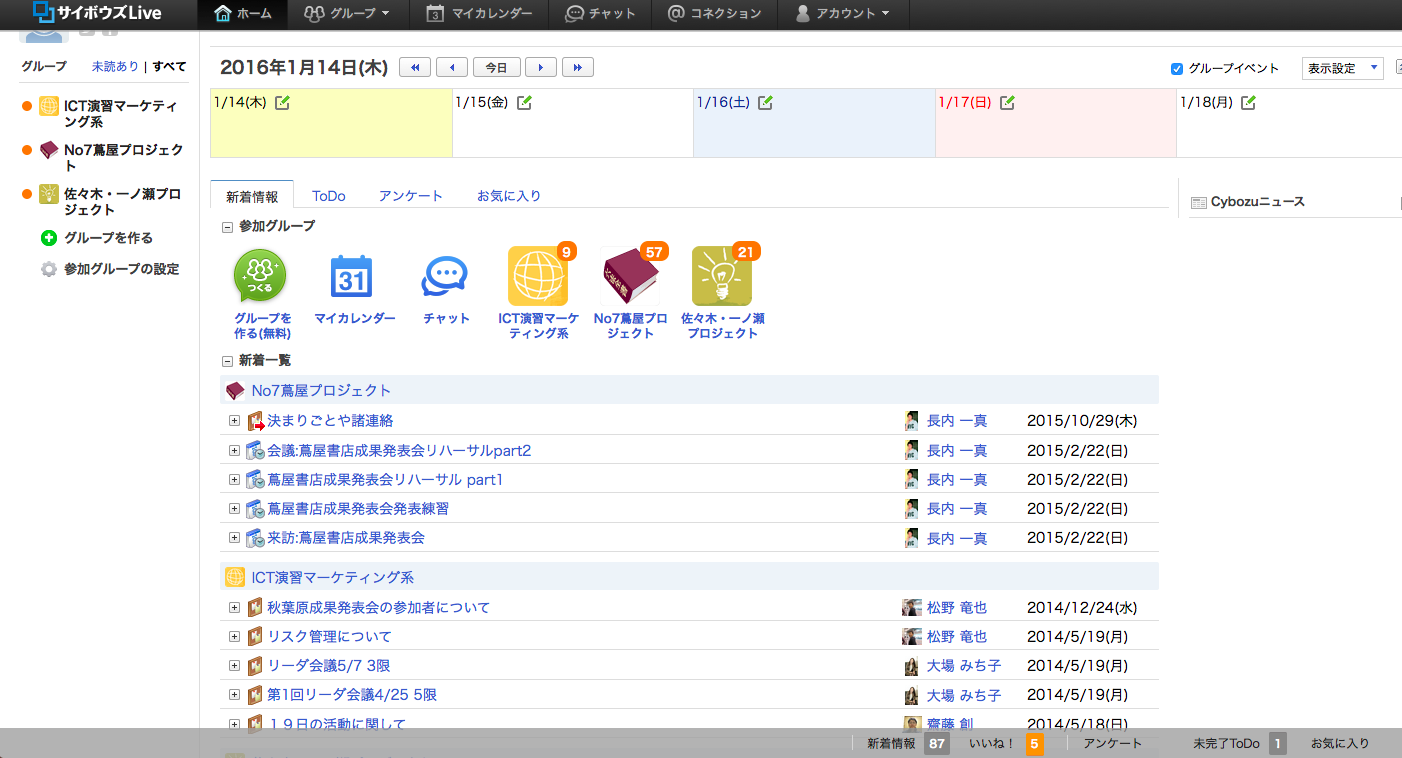
\includegraphics[width=100mm]{./img/cybozulive.png}
 \end{center}
 \caption{サイボウズLive}
 \label{cybozu}
\end{figure}


%--------------------------------------------------------------------
\chapter{提案するアプリケーションの概要}

%この章では,提案する理論,仮説,モデル,アルゴリズム,方法論,実装のなどの説明を行う
提案するアプリケーションは、授業やゼミ等で聞き手が話者にメッセージを発信するための意思決定ツールである. 

\section{提案するアプリケーションの特徴}
%この言語の特徴は,..であり,...という従来にない長所をもつ.
%このアプリケーションの特徴は、クライアント側はLeap Motionを使ってリアルタイムに入力操作を行い、サーバー側に反映するという長所がある.
%このアプリケーションの主な特徴は, Leap Motionを使ってリアルタイムに入力操作を行うことである.
%自分が発信したいメッセージを選択するだけ
%ソケット通信を使って通信を行う。お互いのPCがインターネットに接続されていなければならない。


%ユーザ視点での特徴を丁寧に箇条書き
%機能で説明する
このアプリケーションの特徴は, 主に2つある.\\
 1つ目は, Leap Motionで読み取れる4つのジェスチャーを使い, リアルタイムに入力操作を行うことである. \\
%そもそもの経緯がLeap Motionを使うことにあった
 2つ目は, クライアント側とサーバー側の二つのプログラムに分かれていることである. このアプリケーションでは, クライアント側とサーバー側間のデータを送受信する手段として, ソケット通信を行った. \\
 このアプリケーションの機能は以下のものがある.
\begin{itemize}
 \item ジェスチャーを使ってメッセージを発信する機能
 \item 発信するメッセージに重みをつける機能
 \item 発信されたデータを集計する機能
\end{itemize}

%3つ目は,
%つは,
\subsubsection{全体像}
\begin{figure}[H]
 \begin{center}
  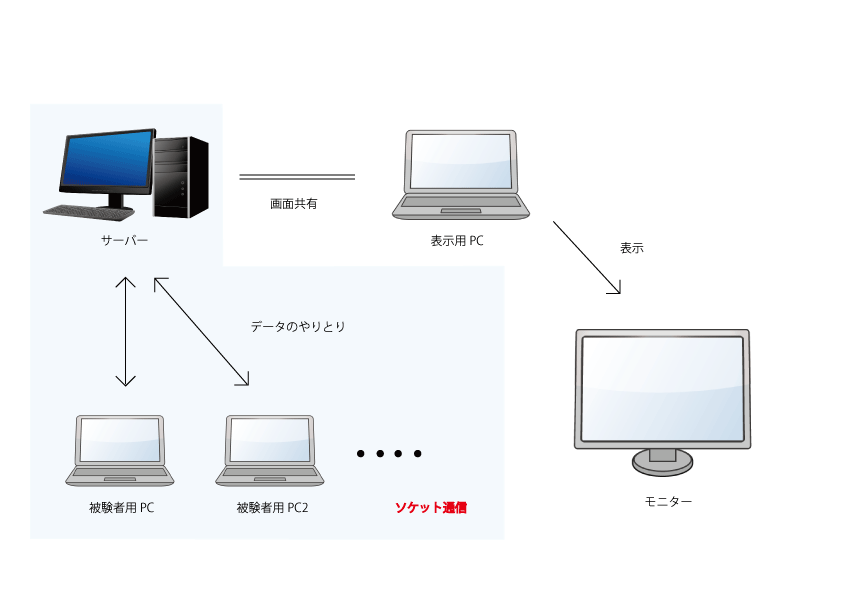
\includegraphics[width=100mm]{./img/zentai.png}
 \end{center}
 \caption{全体像}
 \label{zentai}
\end{figure}

\section{クライアント側のプログラムの役割}
クライアント側は, 聞き手が発信したいメッセージを発信するためのものである. 

\subsubsection{発信する手順}

\begin{enumerate}
 \item ジェスチャーを行い, 入力方法を決める.
 \item ジェスチャーでメッセージの選択を行う.
 \item ジェスチャーの回数で, メッセージに重みをつける.
\end{enumerate}

クライアント側がメッセージを発信する際, 全ての手順をジェスチャーで行うという特徴がある. このように製作した理由は, マウスやキーボードなどの入力装置との差別化を行うためである. 聞き手がメッセージを送信するために行う手順は, 大きく3つある. 
まず, ジェスチャーを行い, 入力方法を決める. 例えば, このときサークルジェスチャーを行った場合, ジェスチャーがメッセージを発信するまでの入力方法になる. 
次に, ジェスチャーでメッセージの選択を行う. 30秒間の時間が設けてあり, 最後に選択されていたメッセージが送信する値になる. このときジェスチャーをするときの指の本数を変える, 選択するメッセージが容易になる. 
最後に, ジェスチャーでメッセージに重みをつける. この段階でも30秒の値が設けてある. ジェスチャーを行った回数で, 自分がどれだけメッセージを伝えたいか発信するメッセージに重みをつけることができる. この回数が次に紹介する各ジェスチャーの値に相当する. 

%どういうメッセージなのか、なぜこのメッセージなのか
%クライアント側からサーバー側のプログラムへ発信される値は以下の5つである. 
%なぜこのような設定になっているのか

\subsubsection{クライアント側から発信する値について}

\begin{itemize}
 \item アカウントナンバー
 \item 手の数
 \item サークルジェスチャーの回数
 \item スワイプジェスチャーの回数
  \item スクリーンタップジェスチャーの回数
 \item キータップジェスチャーの回数
 \item  メッセージナンバー
\end{itemize}

発信される値は全部で7つある, これらの値は, カンマで区切られた1つの文字列になり, サーバー側へ発信される(図\ref{send}).\\ 
まず, アカウントナンバーは固定値であり, それぞれの聞き手には予め番号が振り分けられている. これにより誰がどのような値を送ったかを特定しサーバー側で処理する. \\
次に, 手の数は聞き手がLeap Motionに手をかざしているかの判定に使う. 発信されている値が0の時は, 手をかざしていないことを発信し, 0よりも大きい値の時, 聞き手が手をかざしていることを表す. \\
各ジェスチャーの回数は, メッセージに重みをつける際に, 聞き手が行ったジェスチャーの回数である. 発信された値は, サーバー側で処理され, ビジュアルに反映される. 
最後にメッセージナンバーは, 選択したメッセージを表す. 発信するメッセージは9つ用意されており, それぞれ対応した値が発信される. メッセージナンバーは-1と0から8の値で構成されており, -1のときは選択されていないことを表し, 0から8の値ではそれぞれのメッセージ送られる. \\


\begin{figure}[H]
 \begin{center}
  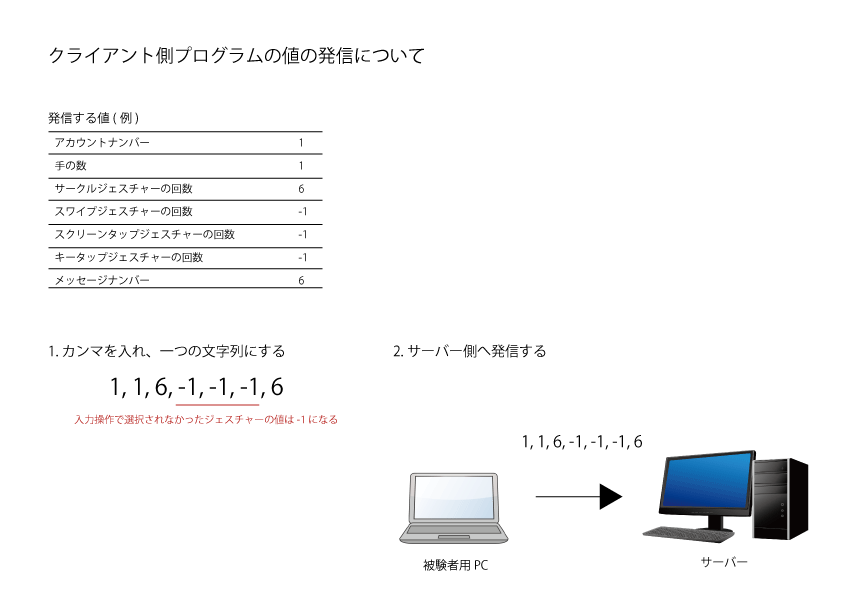
\includegraphics[width=100mm]{./img/sendCL.png}
 \end{center}
 \caption{クライアント側から発信する値}
 \label{send}
\end{figure}


\section{サーバー側のプログラムの役割}

サーバー側では, 聞き手のメッセージを集計し,  その集計結果を発信するためのものである.
まず, 送られてきたメッセージを区切りで分解する. その値を構造体へ代入する. 
\subsubsection{メッセージナンバーの集計}
送られてきたメッセージは構造体へ代入後, どのメッセージが多く発信されたかを算出する. 構造体へ代入されるメッセージナンバーは0から8の値であり, -1のときは代入されない. これにより聞き手が発信した最新のメッセージナンバーが構造体へ代入される. 一番多く受け取ったメッセージナンバーを算出後, その値にあった描写処理を行う.  

\subsubsection{描写処理について}
%どのような描写処理が行われるのか?
聞き手から送られたメッセージに関してまるまるのような描写処理が行われる.聞き手から送られたメッセージに関してまるまるのような描写処理が行われる.聞き手から送られたメッセージに関してまるまるのような描写処理が行われる.聞き手から送られたメッセージに関してまるまるのような描写処理が行われる.聞き手から送られたメッセージに関してまるまるのような描写処理が行われる.聞き手から送られたメッセージに関してまるまるのような描写処理が行われる.聞き手から送られたメッセージに関してまるまるのような描写処理が行われる.

%なぜこのようなUIなのか

\section{実装方法}

\subsection{言語・ツール・開発環境}
使用言語は主にC++である. 一部, C言語での記述もある. IDEはXcodeでLeap Motionを入力装置として使う. また開発環境は表 \ref{env} の通りである. 

\begin{table}[H]
\begin{center}
\caption{開発環境}
  \begin{tabular}{ll}
  
   \hline
OS & OS X  Yosemite Macbook Air \\ 
  \hline
プロセッサ & 1.6 GHz Intel Core i5\\ 
  \hline
メモリ & 4GB 1600 MHz DDR3\\ 
  \hline
  \end{tabular}
  \label{env}
  \end{center}
\end{table}


\subsection{Cinderフレームワークについて}
CinderはC++で書かれたのフレームワークである. 画像や動画, 音声処理に長けており, ライブラリが用意されている. 今回は, アプリケーションの作り方が本で紹介されていたこととCinderを使っての導入事例が多くなってきていることから, Cinderを使って開発を進めることにした. 



\subsubsection{openFrameworksとの違い}
%openFrameworksは創造的なコーディングのためのC++のオープンソースツールキットです
ここではopenFrameworks[]について述べる. openFrameworksはC++のオープンソースツールキットである. openFrameworksは, Cinderと同様に、描写処理等に長けたフレームワークでもあり, Leap Motionを使ったアプリケーションで使われるフレームワークとして、この2つが使われていることが多い. 
openFrameworksはCinderよりも歴史がある. openFrameworksは2004年に開発され広まっていったのに対し. Cinderは2010年から広まった. goolgeトレンド(図\ref{API})では, 近年, Cinderの方がopenFrameworksよりも流行りであることがわかる. 

\begin{figure}[H]
 \begin{center}
  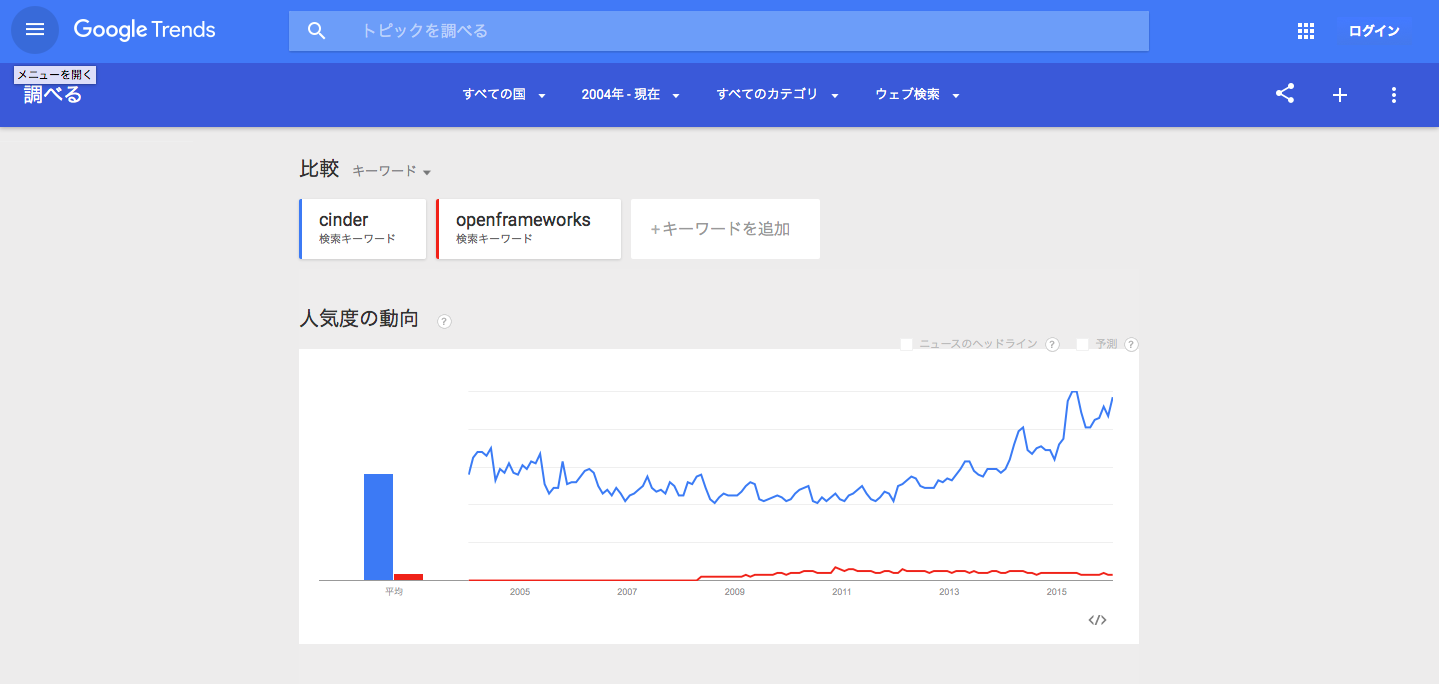
\includegraphics[width=100mm]{./img/api.png}
 \end{center}
 \caption{CidnerとopenFrameworks}
 \label{API}
\end{figure}


\subsection{Leap Motionについて}
%Leap Motionの開発元・リリース時期等を記述.開発言語は
%もっと簡単で良い
Leap Motion(図 \ref{LeapMotion} )とはアメリカのLeap Motion社が2013年にリリースした手や指を検知することに特化したセンサである. Leap Motionは教育や医療など幅広く使われている. 開発のドキュメントとしては, JavaやC++などの6つが用意されている(図 \ref{Leapdoc}参照).



\begin{figure}[H]
 \begin{center}
  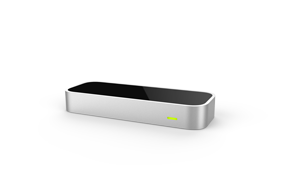
\includegraphics[width=100mm]{./img/LeapMotion.png}
 \end{center}
 \caption{Leap Motion}
 \label{LeapMotion}
\end{figure}

\begin{figure}[H]
 \begin{center}
  
\includegraphics[width=100mm]{./img/Leapdoc.png}
 \end{center}
 \caption{開発ドキュメント}
 \label{Leapdoc}
\end{figure}



\subsubsection{Leap Motionの評価}
%Leap Motionの評価
Leap Motionの入力装置としての特性を追求した. ここではLeap Motionの良い点と欠点をあげる. Leap Motionの良い点は, 3つある. \\ 
 1つ目は, Leap Motionでは手や指の位置や方向, ジェスチャーなどを検知し, リアルタイムで入力操作ができるという点である. ジェスチャーは4種類あり, 以下に示す. 先にも述べたが今回のアプリケーションではサークルジェスチャーとスクリーンタップジェスチャーの2種類を検知する. \\

\begin{itemize}
 \item サークルジェスチャー:スクリーンに向かって円を描くジェスチャー(図 \ref{circle})
 \item スクリーンタップジェスチャー:スクリーンに向かってタップするジェスチャー(図 \ref{sctap})
 \item スワイプジェスチャー:スクリーン方向にスワイプするジェスチャー(図 \ref{swipe})
 \item キータップジェスチャー:Leap Motion方向にタップするジェスチャー(図 \ref{keytap})
\end{itemize}

\begin{figure}[H]
 \begin{minipage}{0.5\hsize}
  \begin{center}
  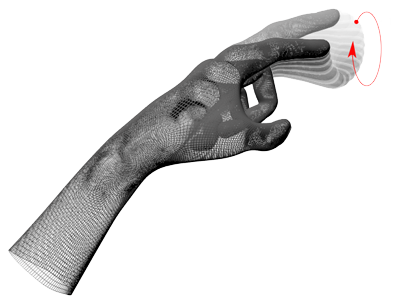
\includegraphics[width=50mm]{./img/Circle.png}
  \end{center}
  \caption{サークルジェスチャー}
  \label{circle}
 \end{minipage}
 \begin{minipage}{0.5\hsize}
  \begin{center}
  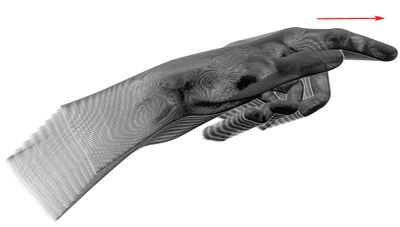
\includegraphics[width=50mm]{./img/ScTap.png}
  \end{center}
  \caption{スクリーンタップジェスチャー}
  \label{sctap}
  \end{minipage}
\end{figure}

\begin{figure}[H]
 \begin{minipage}{0.5\hsize}
  \begin{center}
  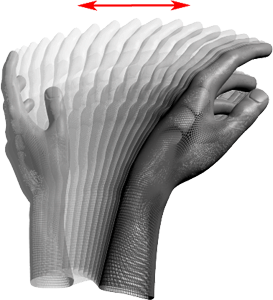
\includegraphics[width=50mm]{./img/Swipe.png}
  \end{center}
  \caption{スワイプジェスチャー}
  \label{swipe}
 \end{minipage}
 \begin{minipage}{0.5\hsize}
  \begin{center}
  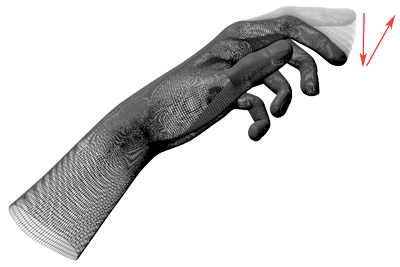
\includegraphics[width=50mm]{./img/KeyTap.png}
  \end{center}
  \caption{キータップジェスチャー}
  \label{keytap}
 \end{minipage}
\end{figure}
%引用元を記述(SDKでいい)

 
  2つ目は, 指の曲げを判定できるので, 入力パターンが豊富であることがいえる. Leap Motionはどの指が曲げられているか, 曲げられている本数は何本か, どのくらい曲げられているか判定することができる. また, 右手と左手の判定もできるので, 以上のことを使えば入力パターンを増やすことが可能である. \\
  3つ目は, Leap Motionをキーボードやマウスなどの入力装置と比較したとき, 音を出さずに入力できるという利点がある. キーボードやマウスにはボタンがあり, 押すとカチッと音がなる. しかし, Leap Motionは指の曲げやジェスチャー等が入力操作として扱われるので音が出ることはない. \\
  一方で, Leap Motionの欠点として次の2つのことを述べる.\\
  1つ目は, センサに不得意な方向があることである. Leap Motionは赤外線センサーで感知しており,  図\ref{leap}のような逆四角錐の範囲で検知される. そのため手を地と垂直に向けると手のひらで指を隠してしまうため, 誤検知される危険性がある. よって, 意識して地と平行にかざすことでLeap Motionが誤操作が発生しにくいことがわかった.\\
  もう1つは, 複数接続が不可能であることである. 1台のPCに接続できるのは1つのLeap Motionで, 2つ以上繋いだ場合, 1台目のLeap Motionが優先され, 2台目は機能しないことがわかった.\\
 
 \begin{figure}[H]
 \begin{center}
  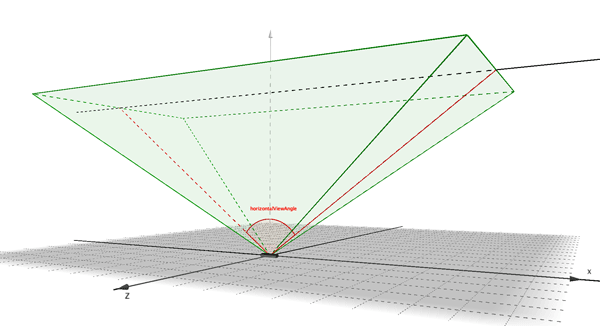
\includegraphics[width=100mm]{./img/LeapAngle.png}
 \end{center}
 \caption{Leap Motionのセンサ範囲}
 \label{leap}
\end{figure}



\subsubsection{ソケット通信について}
%ソケット通信とは。なぜ、どういう意図で通信するのか
%ソケット通信:ソケットというプログラム間でデータの送受信を行うための標準的なプログラムインタフェース(API)を使ってプログラム同士で通信を行うことを指す


%--------------------------------------------------------------------
%全体を通して(1/12)
%受講者は発表者に何が伝えられるのか。通信することによって何がおこるのか。何を起こしたいのかについて詳しく述べるべき。

%--------------------------------------------------------------------
\chapter{実験と評価}

\section{実験について}

ここでは,FUNを用いて記述した場合と
それ以外の言語で書いた場合の比較を行なう.

%\subsection{Fortranとの比較}
%同一のゲームをFortranとFUNで記述してみた.

%\subsubsection{スーパーマリオブラザーズ}
%一見,このプログラムはFortran向きと考えられるが,FUNのTAKOIKAライブラリを用いて記述すると,非常にコンパクトになる.

%\subsubsection{パックマン}

%このプログラムはどちらの言語にとっても,有利な要素はない,このことを反映して.

\subsection{目的}

%Java言語との比較では,惨敗であり,FUNは2倍の記述量を必要とした.しかし,これは,JavaのもつパッケージIKURAが非常に強力であるためで,同一機能をもつライブラリを用意することにより,FUNにも同様の能力を持たせることができることが判明した.

%\section{実行速度}

%\subsection{Fortranとの比較}

%Java言語との比較では,惨敗であり,FUNは2倍の記述量を必要とした.しかし,これは,JavaのもつパッケージIKURAが非常に強力であるためで,同一機能をもつライブラリを用意することにより,FUNにも同様の能力を持たせることができることが判明した.

%\subsection{Javaとの比較}

%Java言語との比較では,惨敗であり,FUNは2倍の記述量を必要とした.しかし,これは,JavaのもつパッケージIKURAが非常に強力であるためで,同一機能をもつライブラリを用意することにより,FUNにも同様の能力を持たせることができることが判明した.

\section{方法}
\subsection{日時と場所}

本実験は丸月丸日, 公立はこだて未来大学の何処何処でおこなった. 

\subsection{被験者}
被験者は公立はこだて未来大学の大学生6人で, 男性が何人, 女性が何人である. 

\subsection{道具}
必要な道具は表\ref{tools}のとおりである

\begin{table}[H]
\begin{center}
\caption{実験器具}
  \begin{tabular}{ll}
   \hline
   道具名 & 台数\\
   \hline
   被験者用Macbook & 6台\\
   \hline
   Leap Motion & 6台\\ 
   \hline
   表示用のMacbook & 1台\\ 
   \hline
  サーバー & 1台\\ 
   \hline
   \end{tabular}
   \label{tools}
  \end{center}
\end{table}

\subsection{配置}
道具は図のように配置する. \\

ここに図を入れる.\\

表示用のは話し手に見えるように配置する.

\subsection{手順}
まず, 被験者全員にクライアント側のプログラムを配布する.\\
サーバー側のプログラムを起動する. \\
被験者はゼミが始まると同時にプログラムを起動してもらう. \\
被験者には伝えたいメッセージがあるときにアプリケーションを使って発信してもらう. \\


%\subsection{初心者}

%Java言語との比較では,惨敗であり,FUNは2倍の記述量を必要とした.しかし,これは,JavaのもつパッケージIKURAが非常に強力であるためで,同一機能をもつライブラリを用意することにより,FUNにも同様の能力を持たせることができることが判明した.

%\subsection{上級者}

%Java言語との比較では,惨敗であり,FUNは2倍の記述量を必要とした.しかし,これは,JavaのもつパッケージIKURAが非常に強力であるためで,同一機能をもつライブラリを用意することにより,FUNにも同様の能力を持たせることができることが判明した.

%--------------------------------------------------------------------
\chapter{考察}

\section{評価結果}

%Java言語との比較では,惨敗であり,FUNは2倍の記述量を必要とした.しかし,これは,JavaのもつパッケージIKURAが非常に強力であるためで,同一機能をもつライブラリを用意することにより,FUNにも同様の能力を持たせることができることが判明した.

\section{評価結果}

%Java言語との比較では,惨敗であり,FUNは2倍の
%記述量を必要とした.しかし,これは,Javaのもつ
%パッケージIKURAが非常に強力であるためで,
%同一機能をもつライブラリを用意することにより,
%FUNにも同様の能力を持たせることができることが判明した.


%--------------------------------------------------------------------
\chapter{結論と今後の展開}

\section{まとめ}

%Java言語との比較では,惨敗であり,FUNは2倍の記述量を必要とした.しかし,これは,JavaのもつパッケージIKURAが非常に強力であるためで,同一機能をもつライブラリを用意することにより,FUNにも同様の能力を持たせることができることが判明した.

%Java言語との比較では,惨敗であり,FUNは2倍の記述量を必要とした.しかし,これは,JavaのもつパッケージIKURAが非常に強力であるためで,同一機能をもつライブラリを用意することにより,FUNにも同様の能力を持たせることができることが判明した.

%Java言語との比較では,惨敗であり,FUNは2倍の記述量を必要とした.しかし,これは,JavaのもつパッケージIKURAが非常に強力であるためで,同一機能をもつライブラリを用意することにより,FUNにも同様の能力を持たせることができることが判明した.

\section{今後の方針}

%Java言語との比較では,惨敗であり,FUNは2倍の記述量を必要とした.しかし,これは,JavaのもつパッケージIKURAが非常に強力であるためで,同一機能をもつライブラリを用意することにより,FUNにも同様の能力を持たせることができることが判明した.


%--------------------------------------------------------------------
\chapter*{謝辞}

謝辞を書く.


%--------------------------------------------------------------------
% 参考文献
\begin{thebibliography}{9}
 \bibitem {A1} 著者, 「タイトル」, 2003.
\end{thebibliography}


% 以降,付録(付属資料)であることを示す
\appendix

%--------------------------------------------------------------------
\chapter*{付録その1} % \chapter{}を使うと「付録A ***」となる

付録その1(プログラムのソースリストなど)を必要があれば載せる

%--------------------------------------------------------------------
\chapter*{付録その2}
\subsubsection{Leap Motionを使用するために}
%インストール方法を記述
Leap Motionを使用するために, まず自身のPCにインストーラがインストールされていなければならない. ここではその手順を示す.\\
%置き方、必要なこと、設定方法などを記述
%必要なこと
%インストーラをダウンロード
%解凍 → こうなったらOK

%設定方法
%操作の高さの調節、道具、etc...

%置き方
%パソコンに対して垂直に置くようにする ← 図が必要!!
%注意ごと(一度手をさし出した向きを変えないこと、できるだけ触れないこと)

Leap Motionを使うためには、3つの手順が必要である. 
\begin{enumerate}
 \item インストーラを公式ホームページのセットアップ(図 \ref{setup})からダウンロードする.
 \item ダウンロードしたものを解凍する. 図 \ref{install} のような画面が表示されるので, 指示に従ってインストールする. 
 \item メニューバーにアイコン(図 \ref{setting} )が表示されていたら完了. 
\end{enumerate}

\subsubsection{Leap Motionを使用する前の確認事項}
Leap Motionのアプリケーションを使用する前に確認しておくべきことを2つあげる. 以下に述べることはLeap Motionのアイコン(図 \ref{setting})から設定を選択しLeap Motionの設定画面(図\ref{Lset})から確認することができる. これらの設定後, Visualizer等で確認するとなお良い. \\
 1つは, 操作の高さを調節しておくことである. Leap Motionでは自動調節機能があり, 操作の高さが可変になるが, 初めてLeap Motion使うとこれに気づきにくい. 実際に使ってもらい, 手が疲れるという声があった. ユーザーによって使いやすさに違いが出るので確認しておくべきである. \\
 もう1つは, 道具の設定がオフになっているかどうかを確認することである. Leap Motionではペンなど棒状の道具を検知できる. 今回のアプリケーションでは, 道具を使って操作することを想定しなかったため, 道具の検知を行っていない. もし, 道具を使ってのアプリケーションを製作する場合では, チェックされていないと検知できないため確認する必要がある. \\

\begin{figure}[H]
 \begin{center}
  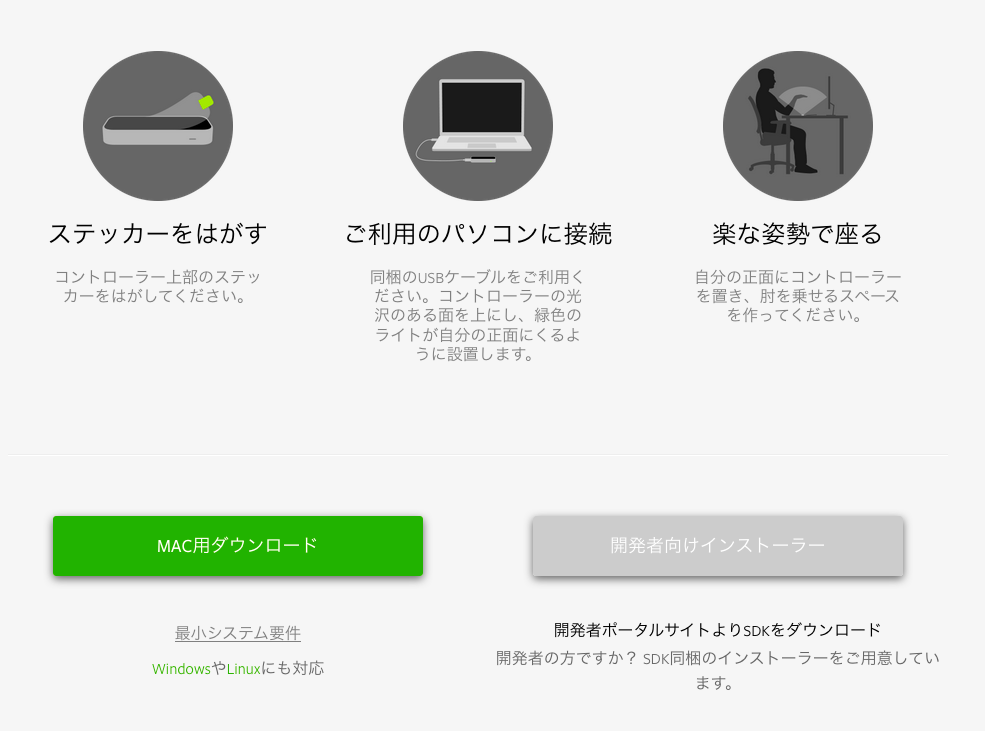
\includegraphics[width=100mm]{./img/setup.png}
 \end{center}
 \caption{Leap Motionのセットアップ}
 \label{setup}
\end{figure}

\begin{figure}[H]
 \begin{center}
  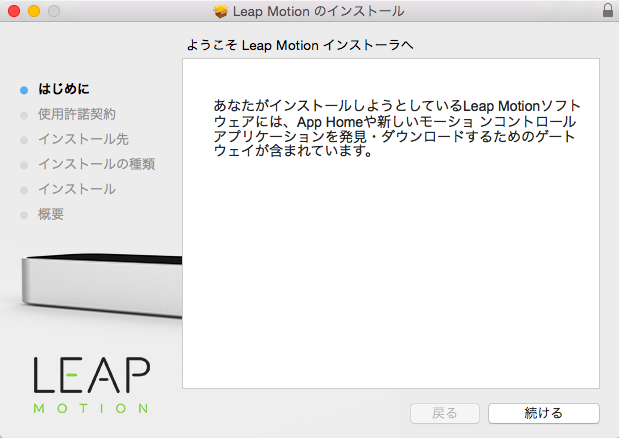
\includegraphics[width=100mm]{./img/installer.png}
 \end{center}
 \caption{インストール画面}
 \label{install}
\end{figure}

\begin{figure}[H]
 \begin{center}
  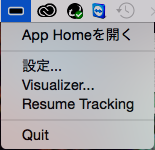
\includegraphics[width=100mm]{./img/setting.png}
 \end{center}
 \caption{Leap Motionのアイコン}
 \label{setting}
\end{figure}

\begin{figure}[H]
 \begin{center}
  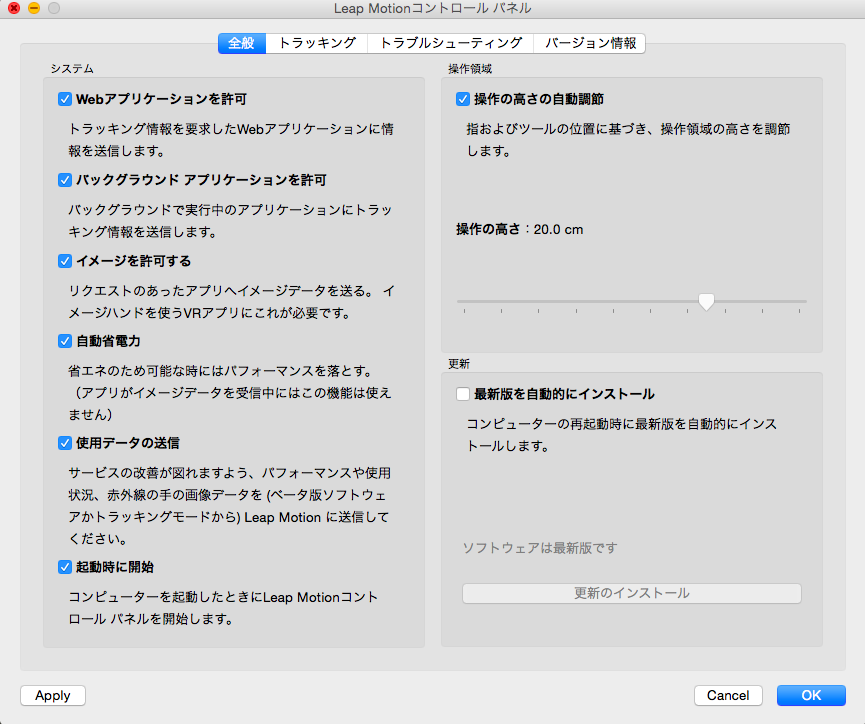
\includegraphics[width=100mm]{./img/Lset.png}
 \end{center}
 \caption{Leap Motionの設定画面}
 \label{Lset}
\end{figure}

\subsubsection{Leap MotionSDKのダウンロード}
Leap Motionを使ったアプリケーションを開発するためにSDKを自分のPCにインストールする必要がある. Leap MotionSDKもLeap Motionインストーラーと同様に, 公式ホームページのセットアップ(図 \ref{setup})よりダウンロードできる. 

%--------------------------------------------------------------------
% 図一覧
\listoffigures

%--------------------------------------------------------------------
% 表一覧
\listoftables

\end{document}